\section{Fick deine Mutter}

Abbildung~\ref{5analysestufen} zeigt schematisch das Vorgehen bei der Risikoanalyse. Es gilt als erstes die zu schützenden \textit{Werte zu identifizieren}. Danach ermittelt man die \textit{Bedrohungen}, welche für die vorher ermittelten Werte bestehen. Anschließend müssen die \textit{Schwachstellen} identifiziert werden, durch welche die Bedrohung wirksam werden kann. Anschließend kann man die \textit{Risiken bewerten} mittels der Formel
\\\\
$ Risiko = Bedrohung * Schwachstelle * Wert $
\\\\
und entsprechende \textit{Prioritäten setzten}, was geschützt werden muss. Ist dies geschehen, kann man entsprechende \textit{Gegenmaßnahmen finden}.



\begin{figure}[h]
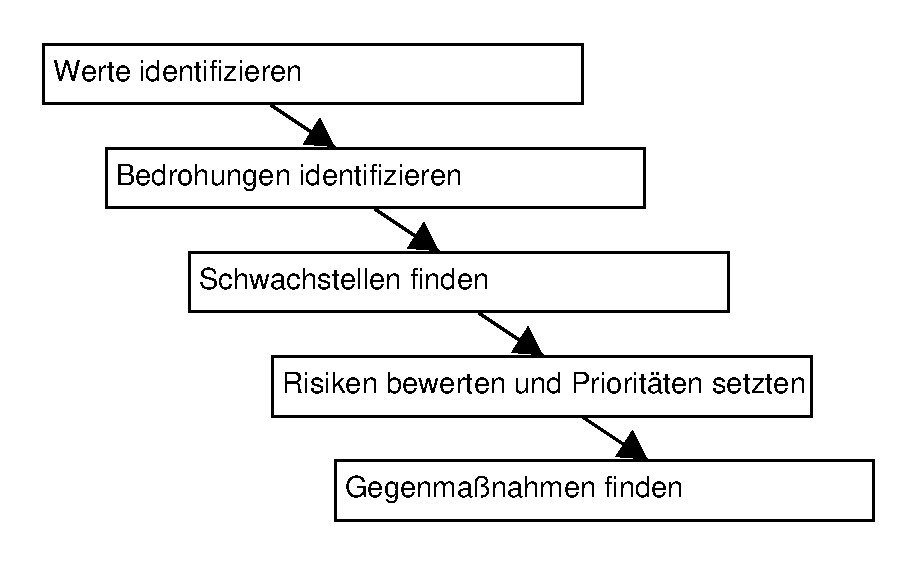
\includegraphics[scale=0.8]{images/5analysestufen.pdf}
\caption{Schematisches Vorgehen bei der Risikoanalyse}
\label{5analysestufen}
\end{figure}

